\section{1D column}

File: \texttt{01\_column.yaml}

\subsection{Description}

The first example is inspired by a real locality of a water treatment
plant tunnel Bedřichov in the granite rock massif. There is a particular
seepage site 23 m under the surface which has a very fast reaction on
rainfall events. Real data of discharge and concentration of stable
isotopes are used.

The user will learn how to:

\begin{itemize}
\tightlist
\item
  Set up the mesh and flow model input parameters;
\item
  Set up the solver and output parameters.
\end{itemize}

A pseudo one-dimensional model is considered in the range 10 \(\times\)
23 m with the atmospheric pressure on the surface and on the bottom, and
no flow boundary condition on the edges (Figure \ref{fig:column_geom}).

\begin{figure}[htbp]
\centering
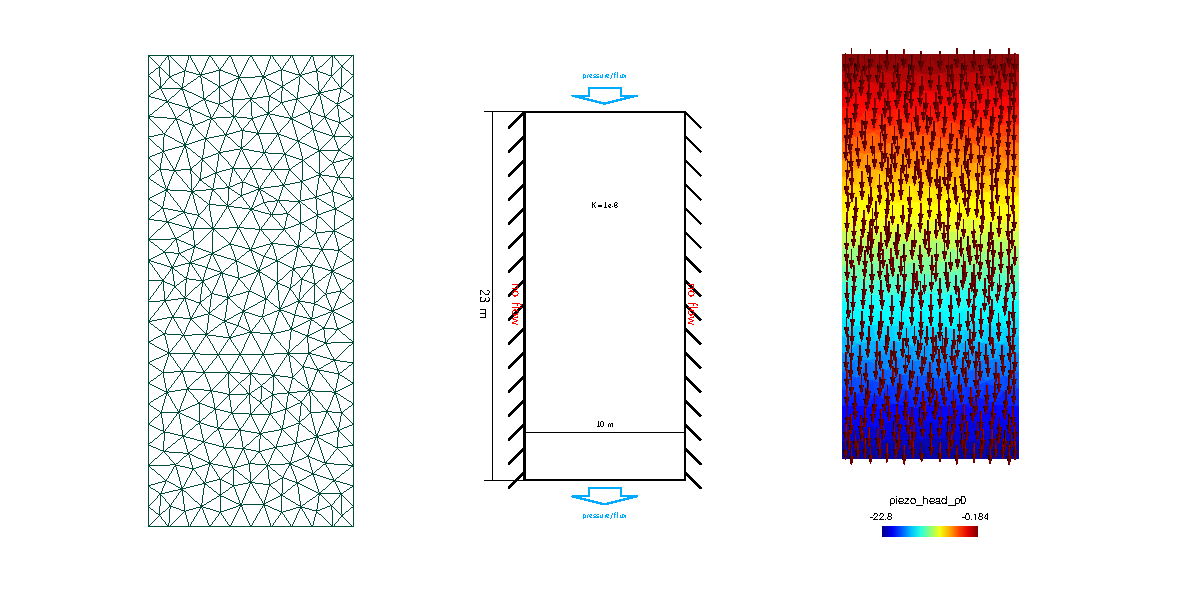
\includegraphics[width=1.00000\textwidth]{tutor_figures/01_mesh_bc_flux.pdf}
\caption{a) the mesh; b) the boundary conditions; c) computed
piezometric head and flux.\label{fig:column_geom}}
\end{figure}

\subsection{Input}

The model settings are given in the control file, which is in YAML
format. Every line contains one parameter and its value(s). The
indentation of lines is important, since it indicates the section to
which the parameter belongs.

\subsubsection{Setting the computational mesh}

The mesh file can be generated using the software
\href{http://www.gmsh.info}{GMSH}. It has to contain:

\begin{itemize}
\tightlist
\item
  point coordinates;
\item
  simplicial elements (lines, triangles, tetrahedra). Elements of lower
  dimensions represent fractures or channels;
\item
  physical regions (groups of elements, labeled either by numerical id
  or string caption). Names of regions defining boundary have to start
  by a dot;
\end{itemize}

The mesh file is specified by the following lines:

\begin{verbatim}
  mesh:
    mesh_file: 01_mesh.msh
\end{verbatim}

\subsubsection{Setting the model and physical parameters}

In this example we use the Darcy flow model, which is set by:

\begin{verbatim}
  flow_equation: !Flow_Darcy_MH
\end{verbatim}

Note: The equation name consists of three parts: physical process
(flow), mathematical model (Darcy) and numerical method (MH = mixed
hybrid finite element method).

The bulk parameters and boundary conditions are defined in the section
\texttt{input\_fields}. For the rock massif (\texttt{-\ region:\ rock})
we prescribe the hydraulic conductivity \(K = 10^{-8}\) m/s (typical
value for the granite rock massif):

\begin{verbatim}
  input_fields:
    - region: rock
      conductivity: 1e-8
\end{verbatim}

We prescribe the atmospheric presure both at the surface and the tunnel:

\begin{verbatim}
    - region: .tunnel
      bc_type: dirichlet
      bc_pressure: 0
    - region: .surface
      bc_type: dirichlet
      bc_pressure: 0
\end{verbatim}

If no boundary condition is given then the default ``no flow'' is
applied.

\subsubsection{Setting solver parameters}

For the solution of the linear algebra problem we have to specify solver
type and tolerances for controlling the residual. In
\texttt{flow\_equation} we can use either \texttt{Petsc} solver which
performs well for small and moderate size problems, or \texttt{Bddc} (a
scalable domain decomposition solver). Two stopping criteria can be
given: absolute and relative tolerance of residual.

\begin{verbatim}
  nonlinear_solver:
    linear_solver: !Petsc
      a_tol: 1e-15
      r_tol: 1e-15
\end{verbatim}

The key \texttt{nonlinear\_solver} has further parameters which play
role in other (nonlinear) flow models.

\subsubsection{Setting output}

In the section \texttt{output\_stream} we define the file name and type
(supported types are \texttt{gmsh} and \texttt{vtk}, which can be viewed
by GMSH, ParaView, respectively) to which the solution is saved:

\begin{verbatim}
  output_stream:
    file: flow.msh
    format: !gmsh
      variant: ascii
\end{verbatim}

The list of fields (solution components, input fields etc.) to be saved
is specified by:

\begin{verbatim}
  output:
    fields:
      - piezo_head_p0
      - pressure_p0
      - pressure_p1
      - velocity_p0
\end{verbatim}

The above code can be alternatively written in a more compact form,
namely

\begin{verbatim}
  output:
    fields: [piezo_head_p0, pressure_p0, pressure_p1, velocity_p0]
\end{verbatim}

In addition to the output of solution, Flow123d provides computation of
balance of fluid volume, flux through boundaries and volume sources.
This is turned on by

\begin{verbatim}
  balance: {}
\end{verbatim}

\subsection{Results}

The results of computation are generated to the files \texttt{flow.msh}
and \texttt{water\_balance.txt}. From the balance file, one can see that
the input flux on the surface is \(1 \times 10^{-7}\) and the output
flux on the tunnel is \(-1 \times 10^{-7}\) (Table
\ref{tbl:tunnel_water_balance}).

\begin{longtable}[c]{@{}lllrrr@{}}
\caption{Results in \texttt{water\_balanced.txt} (edited table, extract
from the file). \label{tbl:tunnel_water_balance}}\tabularnewline
\toprule
``time'' & ``region'' & ``quantity {[}m(3){]}'' & ``flux'' &
``flux\_in'' & ``flux\_out''\tabularnewline
\midrule
\endfirsthead
\toprule
``time'' & ``region'' & ``quantity {[}m(3){]}'' & ``flux'' &
``flux\_in'' & ``flux\_out''\tabularnewline
\midrule
\endhead
0 & ``rock'' & ``water\_volume'' & 0 & 0 & 0\tabularnewline
0 & ``.surface'' & ``water\_volume'' & 1e-07 & 1e-07 & 0\tabularnewline
0 & ``.tunnel'' & ``water\_volume'' & -1e-07 & 0 & -1e-07\tabularnewline
0 & ``IMPLICIT BOUNDARY'' & ``water\_volume'' & 2.58e-26 & 6.46e-26 &
-3.87e-26\tabularnewline
\bottomrule
\end{longtable}

\subsection{Variant}

Control file \texttt{02\_column\_transport.yaml} contains modified
boundary conditions and solute transport model for the same physical
problem.
